\documentclass{book}
\usepackage{graphicx}
\usepackage[english]{babel}
\usepackage{amsthm}
\usepackage{amssymb}
\usepackage{amsfonts}
\usepackage{mdframed}
\usepackage{physics}
\usepackage{tikz}
\usepackage[a4paper, margin=1in]{geometry}
\geometry{a4paper, margin=1in}
\usepackage{xcolor}
\usetikzlibrary{arrows.meta}
\usetikzlibrary{angles,quotes}
\graphicspath{ {./images/} }
\usepackage{svg}
\usepackage{subcaption}
\usepackage{bm}
\usepackage{empheq}
\usepackage{cancel}
\usetikzlibrary{decorations.text}
\usepackage[most]{tcolorbox}
\usepackage{tensor}
%3D
\usepackage{mathtools}
\usepackage{booktabs}
\usepackage{array}
\newcolumntype{C}{>{$}c<{$}}
\usepackage{tikz-3dplot}
\usepackage{appendix}
\usepackage{pgfplots}
\usetikzlibrary{shapes.geometric}
\usetikzlibrary{calc,patterns,angles,quotes}
%Tikz Library
\usetikzlibrary{angles, quotes, intersections}
\usepackage[bb=dsserif]{mathalpha}
\usetikzlibrary{decorations.pathmorphing}

\tikzset{snake it/.style={decorate, decoration=snake}}

\usepackage{etoolbox} % ifthen
\usepackage[outline]{contour} % glow around text
\usetikzlibrary{calc} % for adding up coordinates
\usetikzlibrary{decorations.markings,decorations.pathmorphing}
\usetikzlibrary{angles,quotes} % for pic (angle labels)
\usetikzlibrary{arrows.meta} % for arrow size
\usepackage{xfp} % higher precision (16 digits?)

\usepackage{tcolorbox}

%https://osl.ugr.es/CTAN/macros/latex/contrib/tcolorbox/tcolorbox.pdf
\tcbuselibrary{breakable}
\tcbset{%any default parameters
	width=0.7\textwidth,
	halign=justify,
	center,
	breakable,
	colback=white    
}

\newenvironment{aside}
{\begin{mdframed}[style=0,%
		leftline=false,rightline=false,leftmargin=2em,rightmargin=2em,%
		innerleftmargin=0pt,innerrightmargin=0pt,linewidth=0.75pt,%
		skipabove=7pt,skipbelow=7pt]\small}
	{\end{mdframed}}

\renewcommand{\cleardoublepage}{\clearpage}

\title{Electromagnetism 2}
\author{Dominik Szablonski}
\newtheorem{law}{Law}
\newtheorem{klaw}{Law}
\newtheorem*{definition}{Definition}
\newtheorem*{theorem}{Theorem}

\pgfplotsset{compat=1.18}
\begin{document}
\maketitle

\tableofcontents

\chapter{Sources of Radiation}
Radiation is the phenomenon of energy being transported to an observer. Radiation must be disconnected from its source. Plane electromagnetic waves satisfy conditions of being radiation, and are thus known as free fields. The source of electromagnetic radiation must be charges as those generate the electric and magnetic fields. However, electromagnetic radiation is only generated through accelerating charges. For a free field, there must be locations where radiation propagates while $\rho = 0$.
\section{Charges}
\subsection{Stationary Charges}
For a stationary charge, we can write,
\begin{align}
	\vb{E} = \frac{1}{4\pi\varepsilon_0}\frac{q(\vb{r} - \vb{r}')}{|\vb{r} - \vb{r}'|^3} \propto \frac{1}{|\vb{r} - \vb{r}'|^2} && \vb{B} & = 0
\end{align}
We can clearly see that a stationary charge cannot radiate as it has no component in $\vb{b}$. Furthermore, the energy flow varies as $\vb{1}{r^2}$, which require $\vb{E}\propto\frac{1}{r}$ and $\vb{B}\propto\frac{1}{r}$ which neither field satisfies.
\subsection{Charges with Uniform Velocity}
We can perform a Lorentz boost in the case of a moving charge,
\begin{equation}
	\vb{E}(\vb{r}) = \frac{q}{4\pi \varepsilon_0}\frac{1-\beta^2}{(1 - \beta^2\sin^2\theta)}\frac{\vu{r}}{|\vb{r}|^2}.
\end{equation}
We find that the electric flux still varies as $\frac{1}{r^2}$, thus cannot . Furthermore, we can move into the charge's rest frame where it still varies as $\frac{1}{r^2}$. This is the case as charge is both a conserved and Lorentz invariant quantity.
\\\\
We could also make the an argument using the Biot-Savarte law,
\begin{equation}
	\vb{B}(\vb{r}) = \frac{\mu_0}{4\pi}\frac{q\vb{v}\cross\vu{r}}{\left|\vb{r}\right|^2}
\end{equation}
which still varies as $\frac{1}{r^2}$. Thus, we require acceleration of the charge for radiation to occur.
\begin{aside}
	The reason we require that the electric field and magnetic field be proportional to $1/r$ is because of energy conservation. Let us recall that
	\begin{equation}
		\vb{S} = \frac{1}{\mu_0}\vb{E}\cross\vb{B}
	\end{equation}
	thus $S \propto EB$. We require,
	\begin{equation}
		\int S\cdot\dd{\vb{A}} = \text{Constant}
	\end{equation}
	for energy conservation. Since $\dd{A} \propto r^2$, we require $S \propto 1/r^2$, and thus $E,B \propto 1/r$.
\end{aside}
\section{Retarded Potentials}
If we recall eqs. \eqref{eq:A} and \eqref{eq:phi} of the sourced potentials, we can analyse more closely the static and dynamic cases to gain more insight into radiation phenomena.
\subsection{Statics}
In the static case, we clearly see that we recover Poisson's equation, which we can solve trivially.
\subsection{Time-Dependent case}
In the time dependent case, we require that the electric field propagates at the speed of light $c$. Thus, we wish to obtain a scalar potential $\phi(\vb{r},t)$ sue to a volume of charge $\rho\dd{V}'$ at $\vb{r}'$. We must use the charge density which existed in that volume at an earlier time $\tau$,
\begin{equation}
	\tau = t - \frac{|\vb{r} - \vb{r}'|}{c}
\end{equation}
where $\frac{|\vb{r} - \vb{r}'|}{c}$ is the time taken for information ot travel from $\vb{r}'$ to $\vb{r}$. We can call $\tau$ the \textit{retarded time}. We can thus write down the retarded potentials,
\begin{align}
	&\phi(\vb{r},t) = \frac{1}{4\pi\varepsilon_0}\int_V \frac{\rho(\vb{r}', \tau)}{|\vb{r} - \vb{r}'|}\dd{V}' \\
	&\vb{A}(\vb{r},t) = \frac{\mu_0}{4\pi}\int_V\frac{\vb{J}(\vb{r}',\tau)}{|\vb{r}- \vb{r}'|}\dd{V}'
\end{align}

\section{Radiation from an accelerated charge}
\subsection{Displaced point charge}
\begin{figure}
	\centering
	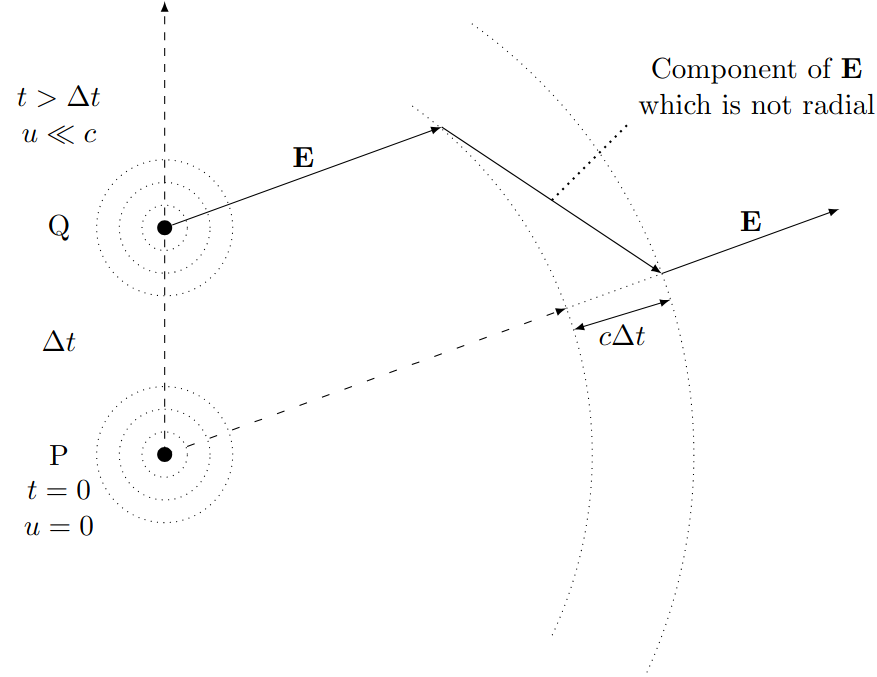
\includegraphics[width=0.75\textwidth]{2.3.png}
	\caption{}
	\label{fig:2.3}
\end{figure}
Consider figure \ref{fig:2.3}, initially at rest at point $P$ in free space. It is given a sudden impulse and undergoes a sudden acceleration $a$ over a short time $\Delta t$, such that when the charge reaches $Q$ it is moving at a constant velocity $u = a\Delta t << c$. If we consider the observer at a far away distance $r$, they will still see the charge at its original, stationary position. In order to see the charge move, the observer must wait a time $t = r/c$. In this time, there must be a boundary where the field configurations move from the old stationary state to the moving state. This boundary will have a width $c\Delta t$ and will must move away from the charge's location at a speed $c$.
\\\\
Let us recall that $\div{\vb{E}} = 0$, so there can be no discontinuities in the field lines generated by the charge. The boundary thus presents itself as a \textit{kink} in the electric field lines, as shown in figure \ref{fig:2.3}. This is a component of $\vb{E}$ which is not radial. 
\begin{figure}
	\centering
	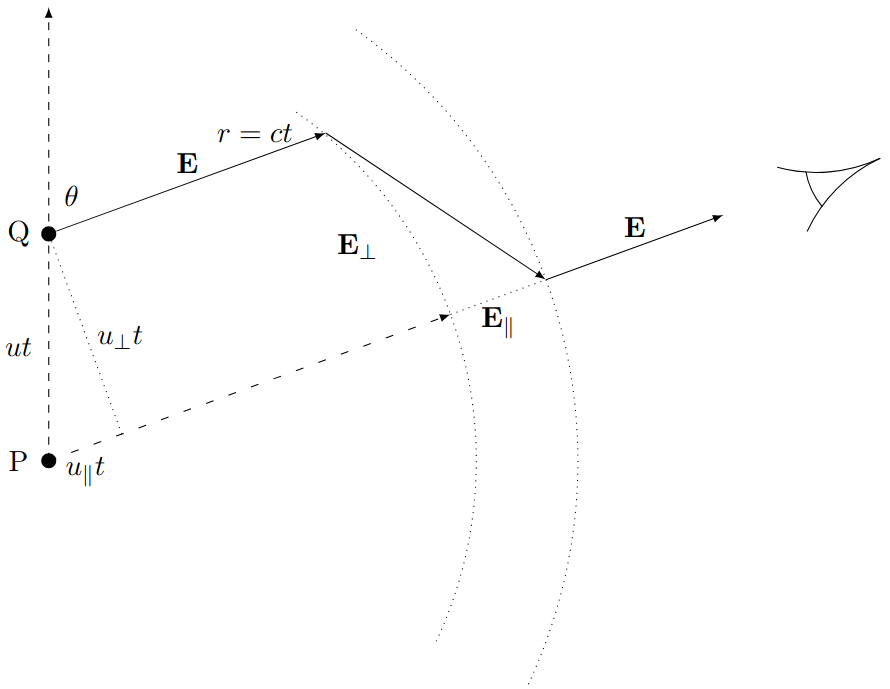
\includegraphics[width=0.75\textwidth]{2.4.png}
	\caption{}
	\label{fig:2.4}
\end{figure}
\\\\
Let us now consider the observer looking at the charge at some angle $\theta$ while it undergoes its final motion, reaching a position $ut$. Let us note that the boundary of observing the charge's motion is
\begin{equation}
	r = ct.
\end{equation}
According to the observer, the charge appears at $u_{\parallel}t$ parallel to their line of sight and  $u_{\perp}t$ perpendicular to their line of sight. We can then relate these to the parallel and perpendicular components of the kink $E_{\parallel}$ and $E_{\perp}$,
\begin{equation}
	\frac{E_{\perp}}{E_{\parallel}} = \frac{u_{\perp} t}{c\Delta t}.
\end{equation}  
If we note that $u_{\perp} = a_{\perp}\Delta t$, we can write,
\begin{equation}
	E_{\perp} = E_{\parallel}\frac{a_{\perp}r}{c^2}.
\end{equation}
Furthermore, since the charge's field is radial, we can say,
\begin{equation}
	E_{\parallel} = \frac{1}{4\pi\varepsilon_0}\frac{q}{r^2}
\end{equation}
so we can write,
\begin{equation}
	E_{\perp} = \frac{1}{4\pi\varepsilon_0}\frac{qa_{\perp}}{c^2r}.
\end{equation}
Let us summarise what we have found using this thought experiment,
\begin{enumerate}
	\item The field $E_{\perp} \propto 1/r$ in the kink region.
	\item Recalling equation \eqref{eq:A4}, we see $B_{\perp} = E_{\perp}/c$ in the kink region.
	\item The magnitude of the Poynting vector $\vb{S} = \frac{1}{\mu_0}\vb{E}\cross\vb{B}$ is, $S \propto EB \propto 1/r^2$
\end{enumerate}
which satisfy our conditions for radiation.
\subsection{Radiation pattern from a displaced point charge}
We wish to now consider the electric field and the power flux (Poynting vector) as time dependent functions, noting that we will require using the retarded time. By noting that $a_{\perp} = a \sin\theta$, we can simply write,
\begin{equation}
	\abs{\vb{E}(\vb{r},t)} = \frac{1}{4\pi\varepsilon_0}\frac{q\abs{\vb{a}\left(t - \frac{r}{c}\right)}\sin\theta}{c^2r}.
\end{equation}
Then, we can write the Poynting vector as,
\begin{equation}
	\abs{\vb{S}(\vb{r},t)} = \frac{1}{16\pi^2\varepsilon_0}\frac{q^2\abs{\vb{a}^2\left(t - \frac{r}{c}\right)}\sin^2\theta}{c^3r^2}.
\end{equation}
\appendix
\chapter{Revision Equations}
\section{Potentials}
\begin{tcolorbox}[colback=red!5!white,colframe=red!75!black,title=Static Electric Potential]
	\begin{align}
		\vb{E} &= - \grad \phi \\
		\laplacian{\phi} &= - \frac{\rho}{\varepsilon_0}
	\end{align}
\end{tcolorbox}
\begin{tcolorbox}[colback=blue!5!white,colframe=blue!75!black,title=Static Magnetic Potential]
	\begin{align}
		\vb{B} &= \curl{\vb{A}} \\
		-\curl{\vb{B}} &= \laplacian{\vb{A}} = - \mu_0 \vb{J}
	\end{align} 
	if we choose,
	\begin{align}
		\vb{A} \to \vb{A} + \grad{\psi} && \div{\vb{A}} = 0.
	\end{align}
\end{tcolorbox}
\begin{tcolorbox}[colback=green!5!white,colframe=green!75!black,title=Dynamic Potentials]
	\begin{align}
		\laplacian\vb{A} - \mu_0\varepsilon_0 \pdv{\vb{A}}{t} &= - \mu_0 \vb{J} \label{eq:A} \\
		\laplacian\vb{\phi} - \mu_0\varepsilon_0\pdv{\phi}{t} &= -\frac{\rho}{\varepsilon_0} \label{eq:phi}
	\end{align}
\end{tcolorbox}
\section{Gauges}
\begin{tcolorbox}[colback=red!5!white,colframe=red!75!black,title=Coloumb Gauge]
	\begin{equation}
		\div{\vb{A}} = 0
	\end{equation}
\end{tcolorbox}
\begin{tcolorbox}[colback=blue!5!white,colframe=blue!75!black,title=Lorenz Gauge]
	\begin{equation}
		\div{\vb{A}} + \frac{1}{c^2}\pdv{\phi}{t} = 0
	\end{equation}
\end{tcolorbox}
\section{Vector Identities}
\begin{tcolorbox}[colback=blue!5!white,colframe=blue!75!black,title=Laplacian of a Vector]
	\begin{equation}
		\curl{\curl{\vb{A}}} = \grad\left(\div{\vb{A}}\right) - \laplacian{\vb{A}}
	\end{equation}
\end{tcolorbox}
\section{EM Waves}
\begin{tcolorbox}[colback=red!5!white,colframe=red!75!black,title=Relation between $\vb{E}$ and $\vb{B}$]
	\begin{equation}
		\vb{B} = \frac{1}{c}\hat{\vb{k}}\cross \vb{E}. \label{eq:A4}
	\end{equation}
\end{tcolorbox}
\end{document}
